\documentclass[twocolumn,floatfix,aps,prd,superscriptaddress,nofootinbib]{revtex4-2}

% Engine guard: glyphtounicode and \pdfgentounicode are pdfTeX primitives.
% Under LuaLaTeX/XeLaTeX they are undefined and the run aborts in the preamble.
\usepackage{iftex}
\ifPDFTeX
  \usepackage[utf8]{inputenc}
  \usepackage[T1]{fontenc}
  \usepackage{lmodern}
  \input{glyphtounicode}
  \pdfgentounicode=1
\else
  \usepackage{fontspec}
  \setmainfont{Latin Modern Roman}
  \setsansfont{Latin Modern Sans}
  \setmonofont{Latin Modern Mono}
\fi
\usepackage{graphicx}
\usepackage{amssymb}
\usepackage{amsmath}
\usepackage{xcolor}
\usepackage{hyperref}
\usepackage{placeins}
\usepackage[protrusion=true,expansion=false]{microtype}
\usepackage{tikz}
\usetikzlibrary{positioning,arrows.meta}
\definecolor{figink}{HTML}{1A1A18}
\definecolor{figmuted}{HTML}{5F5D57}

% Half-page figure* strips must ride at the top of a text page, not own a
% float page of their own (the binary paper's Fig. 2 lesson).
\AtBeginDocument{%
  \renewcommand{\dbltopfraction}{0.92}%
  \renewcommand{\dblfloatpagefraction}{0.55}%
  \renewcommand{\textfraction}{0.1}%
  \setcounter{dbltopnumber}{2}%
}

% The appendix's two figures share a float page.  Stock float pages centre
% their floats and spread the slack between them; \packfloatpages stacks them
% from the top at a fixed gap instead (as in the binary paper).  Both the
% single- and double-column sets are set.
\makeatletter
\newcommand{\packfloatpages}{%
  \setlength{\@fptop}{0pt}%
  \setlength{\@fpsep}{12pt}%
  \setlength{\@fpbot}{0pt plus 1fil}%
  \setlength{\@dblfptop}{0pt}%
  \setlength{\@dblfpsep}{12pt}%
  \setlength{\@dblfpbot}{0pt plus 1fil}%
}
\makeatother

\graphicspath{{figures/}{../../../results/spinningwormhole/figures/}}

\hypersetup{
    colorlinks=true,
    linkcolor=blue,
    filecolor=magenta,
    urlcolor=blue,
    citecolor=blue,
}
\urlstyle{same}
\emergencystretch=2em

\begin{document}

% Ragged page bottoms throughout: a column that falls short ends short, instead
% of REVTeX's flush bottom stretching the slack open between paragraphs.
\raggedbottom

\title{Rotation slows the instability of Ellis--Bronnikov wormholes}

\author{Nikita M. Shirokov}
\email{shirokov.nm@phystech.edu}
\affiliation{\textit{Moscow Institute of Physics and Technology, Moscow, Russia}}
\author{Ilya Nachevsky}
\email{ommnammashivaya@gmail.com}
\affiliation{\textit{Higher School of Economics, Moscow, Russia}}
\date{\today}

\begin{abstract}
We present nonlinear 3+1 evolutions of rotating Ellis--Bronnikov wormholes. We construct stationary rotating drainhole solutions with a spectral solver up to an equatorial rotation velocity of $99\%$ of the speed of light, validate the solver against published symmetric solutions, and correct an inconsistency in a published field equation. Perturbed only by truncation error, the evolutions show that rotation slows the radial instability of the static wormhole. Near $30\%$ of the extremal angular momentum the unperturbed throat expands instead of collapsing, rather than the instability disappearing as second-order perturbation theory suggests. From $58\%$ upward we find no evidence of instability over the evolved times; at the fastest spin this holds at three resolutions. Collapsing rotating throats emit an axisymmetric quadrupolar gravitational-wave burst whose energy grows with spin. We also show that second-order perturbative initial data trigger the instability through their own truncation error, so they are unsuitable for stability studies.
\end{abstract}

\maketitle

\section{Introduction}
\label{sec:intro}

The Ellis--Bronnikov wormhole, a throat held open by a phantom scalar field~\cite{ellis1973,bronnikov1973,morris_thorne1988,visser1995}, is unstable: depending on the sign of the perturbation it collapses to a black hole or expands without bound, on a timescale set by the throat radius~\cite{gonzalez2009lin,gonzalez2009,shinkai2002,bronnikov2011,cremona2019}. Nonlinear 3+1 evolutions confirm both branches for the lone throat~\cite{shirokov2026} and carry them into binaries, whose every channel ends in collapse, expansion or a merged horizon within a few dynamical times~\cite{shirokov2026c}. If traversable wormholes are to persist anywhere, something must shut this instability off.

Rotation is the oldest candidate~\cite{matos2006}. Spinning Ellis--Bronnikov solutions are known perturbatively~\cite{kashargin2008} and, beyond perturbation theory, from the elliptic solver of Kleihaus and Kunz~\cite{kleihaus_kunz2014,chew2016}: a family that starts at the static throat and ends, at equatorial rotation velocity $v_e=1$, on an extremal Kerr black hole, the phantom field vanishing in the limit; no closed form exists~\cite{volkov2021}. On the stability side, Azad, Bl\'azquez-Salcedo, Khoo and Kunz~\cite{azad2023,azad2024} carried the radial mode to second order in spin: the static unstable mode weakens, with a positive $O(J^2)$ correction for every asymmetry, while for nearly symmetric wormholes a second unstable mode grows out of a static zero mode. The two modes cross near $30\%$ of the extremal angular momentum, where the quadratic approximation gives out. The authors conjecture that the modes merge there and the instability disappears, as purely imaginary modes do in five dimensions~\cite{dzhunushaliev2013}. Quasinormal modes of the rapidly rotating family have also been computed~\cite{khoo2024}. The charged analogue warns against optimism: there the merged modes continue as a complex pair, growth that oscillates, and the growth rate reaches zero only in the extremal limit~\cite{blazquez2025}. Which continuation rotation takes in four dimensions is a question a perturbative method cannot answer, and, to our knowledge, no rotating wormhole has yet been evolved nonlinearly.

This paper builds the tools for that evolution and takes its first step. We construct two families of backgrounds as exact stationary solutions, distinguished by the asymmetry $\gamma$ between their two ends (defined in Sec.~\ref{sec:model}). The symmetric family ($\gamma=0$), massless when static, is the one with published data, the curves of Ref.~\cite{kleihaus_kunz2014} and the scalar charges of Ref.~\cite{chew2016}, and we use it to validate the solver and the 3D initial data across the spin range. The drainhole family ($\gamma=-\pi$), whose static member is the mass-1 drainhole evolved in Refs.~\cite{shirokov2026,shirokov2026c}, has no published fast-spin data at all; it is the family we evolve. The solver accepts a solution only if it also satisfies identities it does not impose. These checks exposed an error in a published field equation (Sec.~\ref{sec:model:eq12}) and showed that second-order initial data trigger the instability at their own error level (Sec.~\ref{sec:slow}). We then put the backgrounds on the adaptive-mesh-refinement (AMR) evolution grid, verify them at fourth order, and evolve the drainhole at nine spins (Table~\ref{tab:ladder}). We find that rotation slows the collapse, as second-order perturbation theory predicts; that near $30\%$ of the extremal angular momentum the instability changes its end state, the unperturbed throat turning to expansion; and that from $58\%$ upward the throat shows no growth within the converged spans, at $81\%$ over the full run.

Section~\ref{sec:model} gives the family and the corrected field equations; Sec.~\ref{sec:solver} the solver, the validation against the published data, and the map of the parameter space (Table~\ref{tab:backgrounds}); Sec.~\ref{sec:setup} the numerical setup and the runs (Table~\ref{tab:ladder}); Sec.~\ref{sec:slow} the evolutions; Sec.~\ref{sec:conclusions} the conclusions. Appendix~\ref{app:conv} gives the convergence of the evolutions of the slowest- and fastest-spinning models; Appendix~\ref{app:interface} the choice of timestep. We use $G=c=1$; the evolutions use the code units of Refs.~\cite{shirokov2026,shirokov2026c}, with throat parameter $\eta_0=2$ (defined in Sec.~\ref{sec:model}), in which the static drainhole has mass $M=1$.

\section{The spinning wormhole family}
\label{sec:model}

The matter model is that of our previous work~\cite{shirokov2026,shirokov2026c}: Einstein gravity coupled to a phantom scalar field $\psi$,
\begin{equation}
S=\frac{1}{16\pi}\int d^4x\,\sqrt{-g}\left(R+2\,g^{\mu\nu}\partial_\mu\psi\,\partial_\nu\psi\right),
\label{eq:action}
\end{equation}
whose kinetic term has the reversed sign that makes $\psi$ a ghost. This sign lets the scalar's stress tensor violate the null energy condition, which a static traversable throat requires~\cite{morris_thorne1988,visser1995}. Varying the action with respect to the metric and to $\psi$ gives the field equations of the model [Eqs.~(2)--(3) of Ref.~\cite{chew2016}],
\begin{equation}
R_{\mu\nu}=-2\,\partial_\mu\psi\,\partial_\nu\psi,\qquad
\partial_\mu\!\left(\sqrt{-g}\,g^{\mu\nu}\partial_\nu\psi\right)=0:
\label{eq:fieldeqs}
\end{equation}
Einstein's equations with the phantom's stress tensor as source, and the wave equation for the phantom on the curved background. Spinning the wormhole of Refs.~\cite{shirokov2026,shirokov2026c} up requires the stationary rotating solution of the same theory, constructed numerically inside an ansatz with stationarity and axisymmetry built in. We take the ansatz of Refs.~\cite{kleihaus_kunz2014,chew2016}, who first constructed these solutions,
\begin{equation}
\begin{split}
ds^2&=-e^{f}dt^2+p^2e^{-f}\Big[e^{\nu}\left(d\eta^2+h\,d\theta^2\right)\\
&\quad+h\sin^2\!\theta\left(d\varphi-\omega\,dt\right)^2\Big],
\end{split}
\label{eq:metric}
\end{equation}
with $\eta\in(-\infty,\infty)$ and four unknown functions $f$, $p$, $\nu$, $\omega$ of $\eta$ and $\theta$ [Eq.~(4) of Ref.~\cite{chew2016}]. The field equation for $p$ decouples from the others, and its solution with asymptotically flat boundary conditions is $p=1$ [Eqs.~(5)--(6) of Ref.~\cite{chew2016}]; we set $p=1$ from here on.

In the trivial limit $f=\nu=\omega=0$ the spatial metric is $d\eta^2+h\left(d\theta^2+\sin^2\!\theta\,d\varphi^2\right)$ with the fixed $h=\eta^2+\eta_0^2$: $\sqrt{h}$, the radius of the sphere at coordinate $\eta$, never vanishes; its minimum, $\eta_0$ at $\eta=0$, is the throat, the minimal sphere joining the two asymptotically flat ends $\eta\to\pm\infty$, so the spacetime has no center. This choice of $h$ builds the two-ended, horizonless topology into Eq.~\eqref{eq:metric}; conversely, $\eta_0\to0$ closes the throat and lets the same ansatz hold a black hole, which is how extremal Kerr enters in Sec.~\ref{sec:model:eq12}.

Our previous wormhole sits inside this form: with $\omega=\nu=0$ and the closed-form $\arctan$ profile for $f$~\cite{chew2016}, Eq.~\eqref{eq:metric} is the static drainhole of Refs.~\cite{shirokov2026,shirokov2026c}, with $\eta_0=a$ its throat parameter and $\eta$ the isotropic radius used there, unfolded through the throat (Sec.~\ref{sec:setup:id}); $f=0$ gives the massless Ellis wormhole.

Substituting the ansatz~\eqref{eq:metric} into the field equations~\eqref{eq:fieldeqs} reduces them in three steps. We follow the reduction of Kleihaus and Kunz~\cite{kleihaus_kunz2014}, given in full in Sec.~II of Ref.~\cite{chew2016}; equation numbers in brackets below refer to Ref.~\cite{chew2016}. First, the phantom field equation---the wave equation in Eq.~\eqref{eq:fieldeqs}, which stationarity and axisymmetry reduce to a function of $\eta$ alone---integrates in closed form to $\psi=(D/\eta_0)\left[\arctan(\eta/\eta_0)-\pi/2\right]$ [Eqs.~(7)--(9)]: the scalar enters the rest of the problem only through its constant of integration $D$, the scalar charge. Second, because $\partial_\mu\psi$ points along $\eta$, the source term $-2\,\partial_\mu\psi\,\partial_\nu\psi$ survives only in the $\eta\eta$ Einstein equation; each other nontrivial component ($tt$, $t\varphi$, $\theta\theta$, $\varphi\varphi$, $\eta\theta$) is a statement about the metric functions alone, and these organize by order and role. Two are second-order elliptic equations,
\begin{align}
0={}&\partial_\eta\!\left(h s\,\partial_\eta f\right)+\partial_\theta\!\left(s\,\partial_\theta f\right)\nonumber\\
&-h s^3 e^{-2f}\!\left[h(\partial_\eta\omega)^2+(\partial_\theta\omega)^2\right],
\label{eq:feq}\\
0={}&\partial_\eta\!\left(h^2 s^3 e^{-2f}\partial_\eta\omega\right)\nonumber\\
&+\partial_\theta\!\left(h s^3 e^{-2f}\partial_\theta\omega\right),
\label{eq:omeq}
\end{align}
with $s\equiv\sin\theta$ [Eqs.~(10)--(11)]: Eq.~\eqref{eq:feq} is a Laplace-type equation for the redshift $f$, sourced by the squared gradients of the frame dragging (rotation gravitates), and Eq.~\eqref{eq:omeq} is a total divergence, angular-momentum conservation, forcing the same $J$ through every $\eta=\mathrm{const}$ surface. The single off-diagonal component is only first order in $\nu$,
\begin{equation}
\begin{split}
0&=-h s\,\partial_\eta f\,\partial_\theta f+h\cos\theta\,\partial_\eta\nu\\
&\quad+\eta s\,\partial_\theta\nu+h^2 s^3 e^{-2f}\partial_\eta\omega\,\partial_\theta\omega,
\end{split}
\label{eq:constraint}
\end{equation}
so $\nu$ follows by integration once $f$ and $\omega$ are known [Eq.~(13)]. (The remaining diagonal components give a second-order equation for $\nu$, Sec.~\ref{sec:model:eq12}.) Third, the one sourced component, $R_{\eta\eta}=-2D^2/h^2$ [Eq.~(18)], rearranges into an algebraic identity for the charge [Eq.~(19)]: the metric functions fix $D^2$ at every point, so its constancy over the domain is a solution test that comes for free. The system for three unknowns is overdetermined. The Bianchi identities make it consistent on an exact solution, so a numerical scheme must choose which subset to impose, a choice Sec.~\ref{sec:model:eq12} shows matters. The boundary conditions select the family: Minkowski at $\eta\to+\infty$, and $f\to\gamma$, $\omega\to\omega_\infty$ at $\eta\to-\infty$, so the constant $\gamma$ measures how unequal the two ends are and $\omega_\infty$ sets the spin.

A solution of this system is three functions and one number, $(f,\nu,\omega;D)$. Every physical quantity we quote---the columns of Table~\ref{tab:backgrounds}---is read off them directly~\cite{kleihaus_kunz2014,chew2016}:
\begin{itemize}
\item far from the throat the metric settles to the field of a point mass, $f\to-2\mu_+/\eta$ as $\eta\to+\infty$ and $f\to\gamma+2\mu_-/\eta$ as $\eta\to-\infty$, so the end masses $\mu_\pm$ are the $1/\eta$ coefficients of $f$;
\item likewise $\omega\to2J/\eta^3$, and the charges obey the Smarr-type relation $\mu_++\mu_-=2\,\omega_\infty J$~\cite{chew2016};
\item the throat is the sphere of minimal area, at $\eta_t=0$ when the two ends are equal ($\gamma=0$) and displaced toward the positive-mass end otherwise ($\eta_t=\eta_0/2$ for the static drainhole): its equatorial circumference gives the radius $R_e=e^{-f/2}\sqrt{h}\,\big|_{\eta_t,\,\theta=\pi/2}$, its meridians the polar radius $R_p$, its area the areal radius $R_A$---three numbers that coincide while the throat is round and split as rotation flattens it;
\item the throat is dragged at the angular velocity $\Omega=\omega\,\big|_{\eta_t,\,\theta=\pi/2}$, and $v_e=R_e\,\Omega$ is its equatorial linear velocity in units of $c$: the dimensionless spin label used throughout, 0 when static and 1 at the extremal Kerr endpoint.
\end{itemize}

We construct two one-parameter families, labelled by $\omega_\infty$ (equivalently $J$ or $v_e$):
\begin{itemize}
\item[(a)] \emph{the drainhole family}, $\eta_0=2$, $\gamma=-\pi$: its static member, with end masses $\mu_\pm=\pm1$, is the wormhole of Refs.~\cite{shirokov2026,shirokov2026c}; its end-mass asymmetry is $C=1$ in the notation of Refs.~\cite{azad2023,azad2024}.
\item[(b)] \emph{the symmetric family}, $\gamma=0$ ($C=0$), that of Refs.~\cite{kleihaus_kunz2014,chew2016}: equal masses on both ends, the massless Ellis wormhole when static; for the 3D checks it is rescaled $\eta_0\,{=}\,1\to2$, so its throat sits on family (a)'s grid.
\end{itemize}

\subsection{A correction to the published $\nu$ equation}
\label{sec:model:eq12}

Refs.~\cite{kleihaus_kunz2014,chew2016} close the system with a second-order equation for $\nu$, Eq.~(12) of Ref.~\cite{chew2016}. We find that this equation requires a correction. The scalar-free component $R_{\theta\theta}=0$, with the second derivatives of $f$ and $\omega$ eliminated by Eqs.~\eqref{eq:feq}--\eqref{eq:omeq}, gives
\begin{equation}
\begin{split}
0&=\partial_\eta\!\left(h s\,\partial_\eta\nu\right)+s\,\partial_\theta^2\nu-\cos\theta\,\partial_\theta\nu+s\,(\partial_\theta f)^2\\
&\quad-h s^3 e^{-2f}\left[h(\partial_\eta\omega)^2+2(\partial_\theta\omega)^2\right],
\end{split}
\label{eq:nueq}
\end{equation}
where the printed form has $-2(\partial_\theta\omega)^2$ and no $s\,(\partial_\theta f)^2$ term. Extremal Kerr fits the ansatz~\eqref{eq:metric} in closed form (with $\eta_0=0$), and substituted symbolically, at 160-digit arithmetic, it satisfies Eqs.~\eqref{eq:feq}--\eqref{eq:constraint}, Eq.~\eqref{eq:nueq} and the $D^2$ identity exactly, while leaving a residual of up to $0.35$ (at $M=1$) in the printed $\nu$ equation alone. The error also appears numerically: solutions of the printed elliptic system converge at every resolution, yet carry a violation of the unimposed Eq.~\eqref{eq:constraint} and $D^2$ identity that scales as $J^4$ and does not shrink with the grid, the signature of a difference in the continuous equations rather than in the numerics. Our solver imposes neither $\nu$ equation (Sec.~\ref{sec:solver}), and Eq.~\eqref{eq:nueq} holds on all 200 saved solutions of both families to $\le7\times10^{-8}$ of its largest term within 20 throat radii, where the printed form differs by up to $53\%$. Every published conclusion of Refs.~\cite{kleihaus_kunz2014,chew2016} that we can test survives the correction (Sec.~\ref{sec:solver}).

\section{Backgrounds across the spin range}
\label{sec:solver}

\begin{figure*}[t]
\centering
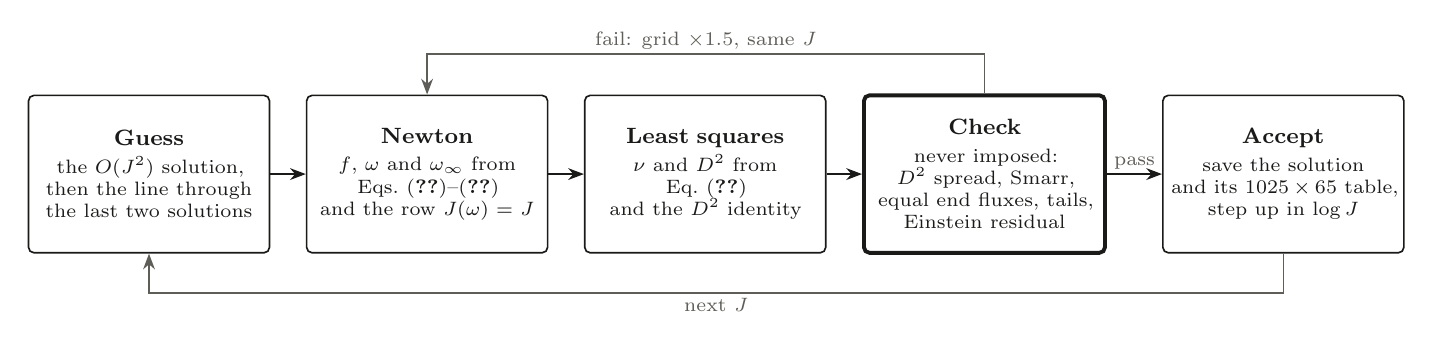
\begin{tikzpicture}[
  font=\scriptsize, node distance=4.5mm,
  box/.style={draw=figink, line width=0.6pt, rounded corners=2pt, align=center,
              text width=28.5mm, minimum height=20mm, inner sep=3pt, text=figink},
  gate/.style={box, line width=1.4pt},
  flow/.style={-{Stealth[length=2mm]}, line width=0.6pt, draw=figink},
  back/.style={-{Stealth[length=2mm]}, line width=0.6pt, draw=figmuted},
  tag/.style={text=figmuted, inner sep=1.5pt}]
\node[box] (seed) {{\footnotesize\bfseries Guess}\\[2pt]
  the $O(J^2)$ solution,\\ then the line through\\ the last two solutions};
\node[box, right=of seed] (newton) {{\footnotesize\bfseries Newton}\\[2pt]
  $f$, $\omega$ and $\omega_\infty$ from\\ Eqs.~(\ref{eq:feq})--(\ref{eq:omeq})\\ and the row $J(\omega)=J$};
\node[box, right=of newton] (nu) {{\footnotesize\bfseries Least squares}\\[2pt]
  $\nu$ and $D^2$ from\\ Eq.~(\ref{eq:constraint})\\ and the $D^2$ identity};
\node[gate, right=of nu] (gates) {{\footnotesize\bfseries Check}\\[2pt]
  never imposed:\\ $D^2$ spread, Smarr,\\ equal end fluxes, tails,\\ Einstein residual};
\node[box, right=7mm of gates] (out) {{\footnotesize\bfseries Accept}\\[2pt]
  save the solution\\ and its $1025\times65$ table,\\ step up in $\log J$};
\draw[flow] (seed) -- (newton);
\draw[flow] (newton) -- (nu);
\draw[flow] (nu) -- (gates);
\draw[flow] (gates) -- node[tag, above] {pass} (out);
\draw[back] (gates.north) -- ++(0,5mm) -| node[tag, pos=0.25, above] {fail: grid $\times1.5$, same $J$} (newton.north);
\draw[back] (out.south) -- ++(0,-5mm) -| node[tag, pos=0.25, below] {next $J$} (seed.south);
\end{tikzpicture}
\caption{The solver loop for one family (Sec.~\ref{sec:solver}). Thin boxes impose equations; the heavy box tests identities the solver never imposes, and only it decides acceptance. A failed check refines the grid and solves the same $J$ again; an accepted solution seeds the next $J$. The loop gave 462 accepted solutions in 20 continuation sweeps, both families to $v_e\approx0.99$.}
\label{fig:solver}
\end{figure*}

\begin{figure}[t]
\centering
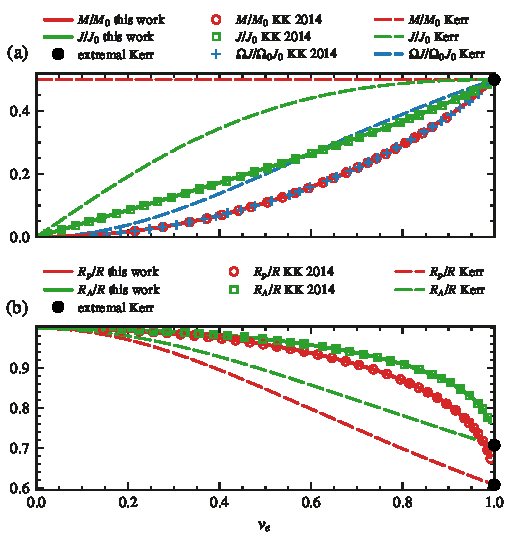
\includegraphics[width=\columnwidth]{solver/kk2014_comparison.pdf}
\caption{The symmetric family ($\eta_0=1$, $\gamma=0$; 81 solutions, $v_e=0.02$--$0.991$, plus the exact static member) in the normalization of Ref.~\cite{kleihaus_kunz2014} ($M_0=R_e$, $J_0=R_e^2/2$, $\Omega_0=1/R_e$): our curves, the digitized points of their Fig.~1 (open symbols), and closed-form Kerr (dashed). The digitization's reading error, measured by reading their printed Kerr curves the same way, is rms $1$--$6\times10^{-4}$; digitized minus ours is rms $2.5$--$8\times10^{-4}$, max $2.5\times10^{-3}$, over all five curves. The two solvers agree to the precision a printed figure carries.}
\label{fig:kk2014}
\end{figure}

\begin{figure*}[t]
\centering
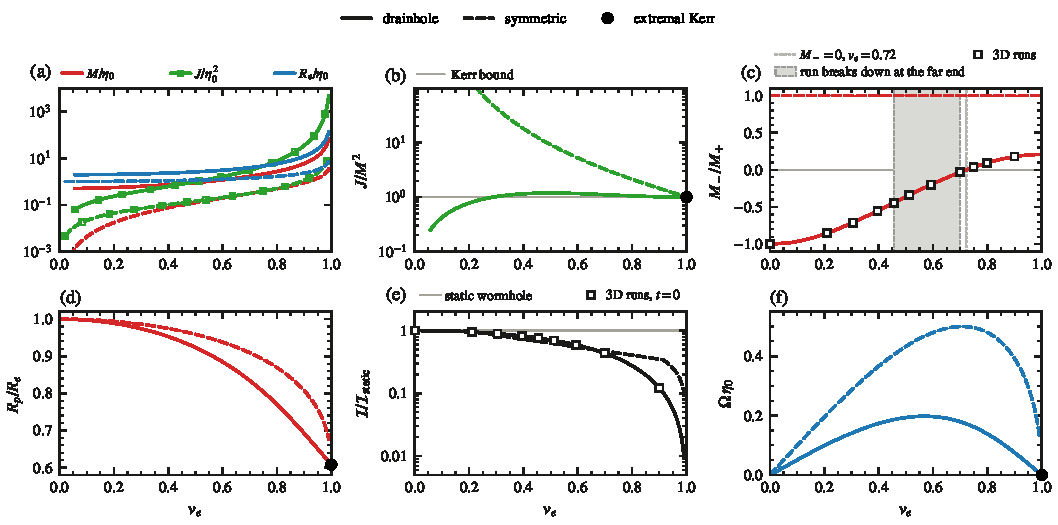
\includegraphics[width=\textwidth]{solver/spin_trends.pdf}
\caption{The drainhole ($\eta_0=2$, $\gamma=-\pi$) and symmetric ($\eta_0=1$, $\gamma=0$) families across the spin range, against $v_e$: (a) the mass $M=\mu_+$ of the $\eta\to+\infty$ end, the angular momentum and the equatorial throat radius; (b) $J/M^2$ against the Kerr bound; (c) the end-mass ratio $M_-/M_+=\mu_-/\mu_+$, which changes sign along the drainhole family at $v_e=0.72$ (dotted), with the backgrounds of the 3D runs (squares); in the shaded band ($v_e=0.46$--$0.70$) the far end has negative mass and the throat does not collapse, and the 3D evolution breaks down before $t=150$ at the puncture $r=0$ into which the far end is compactified; (d) the flattening $R_p/R_e$; (e) the exotic matter: the phantom field's integrated null-energy violation over the $t=\,$const slice per equatorial throat radius, $\mathcal{I}=\int(\rho+p_\eta)\,dV/R_e$~\cite{visser2003} ($\rho$: energy density, $p_\eta$: radial pressure), relative to the static member's $\mathcal{I}_{\rm static}$, with the 3D runs (squares) placed by the scalar charge measured on each run's own $t=0$ slice, which reproduces its background's to $3\times10^{-4}$; (f) the throat angular velocity, which peaks and falls to zero at extremality. Both families end on extremal Kerr, and the faster they spin, the less exotic matter each unit of throat radius needs.}
\label{fig:trends}
\end{figure*}

We solve the system of Sec.~\ref{sec:model} in five steps (Fig.~\ref{fig:solver}):
\begin{enumerate}
\item\emph{Compactify.} The coordinate $x=(2/\pi)\arctan(\eta/\eta_0)$ maps both asymptotic ends to $x=\pm1$, and the unknowns $f$ and $\omega$ are expanded in Chebyshev polynomials of $x$ and even cosine modes of $\theta$.
\item\emph{Solve.} The two elliptic equations~\eqref{eq:feq}--\eqref{eq:omeq} are solved for the expansion coefficients by Newton iteration (guess, linearize, correct) until their residual sits at round-off.
\item\emph{Recover $\nu$ and $D$.} The first-order constraint~\eqref{eq:constraint} and the $D^2$ identity together overdetermine $\nu$ and the single number $D^2$, so both are extracted as one linear least-squares problem, with no second-order $\nu$ equation imposed; the redundancy is a feature, since the leftover misfit measures the error.
\item\emph{Continue in spin.} Every converged solution seeds the Newton iteration at a slightly higher spin, with $J$ as the continuation parameter ($\omega_\infty$ is not monotone along a family), and the grid refines automatically, from $48\times12$ up to $240\times60$, whenever the acceptance checks fail.
\item\emph{Accept.} A solution is kept only if it satisfies five identities the solver never imposes, to the tolerances of Table~\ref{tab:gates}.
\end{enumerate}
The fifth identity, a symbolically generated residual of the full Einstein equations evaluated out to 20 throat radii, is the sharpest. It is $1.0\times10^{-10}$ at $J=0.25$ and $4.2\times10^{-10}$ at $J=1$, against the static member's $2\times10^{-11}$ round-off floor; the $O(J^2)$ perturbative data give $3\times10^{-5}$ and $1\times10^{-2}$ on the same meshes. It stays near $10^{-9}$ up to $v_e\approx0.85$ and reaches ${\sim}10^{-7}$ at $v_e=0.91$--$0.99$. The high-spin $10^{-7}$ is round-off, not solution error: it does not shrink on finer grids, while the global charges agree to 12 digits across them; a deliberately under-resolved solution gives a residual of $10^{-4}$ and is rejected. Beyond 20 throat radii the residual's normalization inflates round-off and the test is switched off; the outer region is covered by the resolution study and the 3D constraint checks of Sec.~\ref{sec:setup}. The resulting global charges agree to 10 digits across three grids, and each background is exported as a $1025\times65$ table whose bilinear interpolation error is $\le10^{-7}$ up to $v_e=0.9$.

\begin{table}[t]
\caption{The acceptance tolerances of step 5: five identities the solver never imposes, and the largest violation an accepted solution may carry. The Einstein residual is evaluated within 20 throat radii; its accepted values are spin-dependent (see text).}
\label{tab:gates}
\begin{ruledtabular}
\begin{tabular}{ll}
identity & tolerance \\
\hline
spread of $D^2$ over the domain & $10^{-11}$ \\
Smarr relation $\mu_++\mu_-=2\,\omega_\infty J$ & $10^{-10}$ \\
equal $J$ flux through the two ends & $1.3\times10^{-9}$ \\
asymptotic tails & $5\times10^{-12}$ \\
Einstein residual & $10^{-10}$--$10^{-7}$ \\
\end{tabular}
\end{ruledtabular}
\end{table}

\begin{table}[t]
\caption{Scalar charge $D$ of the anchor solutions ($\eta_0=1$, $\omega_\infty=0.5$) against Ref.~\cite{chew2016}. Along each fixed-$\gamma$ family, $\omega_\infty$ rises, turns over and descends, so $\omega_\infty=0.5$ is reached twice; the published values sit on the post-turnover branch. Our values are grid-converged to the digits shown; the $\gamma=2$ family continued to $J=172$ confirms no third crossing exists. The pre-turnover branch is new.}
\label{tab:anchors}
\begin{ruledtabular}
\begin{tabular}{llll}
$\gamma$ & $D$ (this work) & $D$~\cite{chew2016} & $D$ (pre-turnover, new) \\
\hline
$-1$ & 0.716368   & 0.71636 & 0.969194 \\
$0$  & 0.552771   & 0.55277 & 0.986013 \\
$1$  & 0.4314654  & 0.43155 & 1.008136 \\
$2$  & 0.3375993  & 0.33984 & 1.048161 \\
\end{tabular}
\end{ruledtabular}
\end{table}

Figure~\ref{fig:kk2014} validates the symmetric family against the published curves. Of the four solutions tabulated in Ref.~\cite{chew2016} at $\omega_\infty=0.5$, two ($\gamma=0,-1$) agree to all printed digits and two ($\gamma=1,2$) differ by $2\times10^{-4}$ and $6.6\times10^{-3}$ from our grid-converged values, consistent with their finite-difference error growing with $\gamma$ (Table~\ref{tab:anchors}).

\begin{table*}[t]
\caption{The two families at representative spins, in units of $\eta_0$: rotation velocity $v_e$, angular momentum, mass of the $\eta\to+\infty$ end, ratio of end masses, scalar charge, equatorial throat radius, flattening, and throat angular velocity---each read off the solution's functions as defined in Sec.~\ref{sec:model}. Every row is a converged solution that passed the acceptance checks of Sec.~\ref{sec:solver}.}
\label{tab:backgrounds}
\begin{ruledtabular}
\begin{tabular}{llllllllll}
family & $v_e$ & $J/\eta_0^2$ & $\mu_+/\eta_0$ & $\mu_-/\mu_+$ & $D/\eta_0$ & $R_e/\eta_0$ & $R_p/R_e$ & $\Omega\,\eta_0$ \\
\hline
(a) drainhole & 0.213 & 0.2535 & 0.5574 & $-0.850$ & 1.1004 & 2.0319 & 0.9873 & 0.1046 \\
              & 0.513 & 1.0278 & 0.9302 & $-0.339$ & 1.0007 & 2.6271 & 0.9194 & 0.1952 \\
              & 0.699 & 3.0417 & 1.6557 & $-0.032$ & 0.8598 & 3.8864 & 0.8351 & 0.1798 \\
              & 0.900 & 34.550 & 5.8400 & $+0.179$ & 0.5327 & 11.911 & 0.6926 & 0.0755 \\
              & 0.950 & 152.16 & 12.316 & $+0.201$ & 0.3785 & 24.751 & 0.6504 & 0.0384 \\
              & 0.990 & 4053.8 & 63.666 & $+0.208$ & 0.1698 & 127.36 & 0.6165 & 0.0078 \\
\hline
(b) symmetric & 0.239 & 0.0542 & 0.0252 & 1 & 0.9881 & 1.0299 & 0.9913 & 0.2323 \\
              & 0.434 & 0.1158 & 0.0906 & 1 & 0.9583 & 1.1101 & 0.9699 & 0.3911 \\
              & 0.667 & 0.2683 & 0.2666 & 1 & 0.8854 & 1.3420 & 0.9197 & 0.4969 \\
              & 0.847 & 0.7007 & 0.6305 & 1 & 0.7653 & 1.8836 & 0.8440 & 0.4499 \\
              & 0.898 & 1.0989 & 0.8685 & 1 & 0.7043 & 2.2722 & 0.8092 & 0.3952 \\
              & 0.952 & 2.4701 & 1.4383 & 1 & 0.5971 & 3.2703 & 0.7539 & 0.2911 \\
              & 0.990 & 12.235 & 3.4312 & 1 & 0.4157 & 7.0595 & 0.6795 & 0.1402 \\
\end{tabular}
\end{ruledtabular}
\end{table*}

Figure~\ref{fig:trends} and Table~\ref{tab:backgrounds} are the map of the parameter space that Refs.~\cite{kleihaus_kunz2014,chew2016} left open, including the massive drainhole family, from which binaries can be built~\cite{shirokov2026c}. Two of its features matter later. First, both families violate the Kerr bound (Fig.~\ref{fig:trends}b): the symmetric family at every spin, with $J/\mu_+^2\approx85$ already at $v_e=0.24$, falling monotonically to 1 at extremality since its static member is massless, and the drainhole family by up to ${\sim}20\%$ at intermediate spin. A collapsing overspun throat cannot settle to a Kerr black hole of the same mass and spin, which makes these backgrounds natural initial data for tests of cosmic censorship. Second, the drainhole's negative far-end mass $\mu_-$ rises through zero at $v_e\approx0.7$: above that spin both ends have positive mass. The exotic matter per throat radius falls a hundredfold along the drainhole family and tenfold along the symmetric one by $v_e=0.99$ (Fig.~\ref{fig:trends}e).

\section{Numerical setup}
\label{sec:setup}

\begin{table}[t]
\caption{The simulations: the drainhole family (a), in code units. Model D$n$ is the drainhole background with $v_e\approx n/100$ (D0: static); D21$\pm\varepsilon$ carries an imposed radial perturbation $|\varepsilon|=10^{-3}$, outward and inward. $8\pi J/A$ is the angular momentum as a percentage of its extremal value $J_{\rm ext}=A/8\pi$ at the throat area $A$, and $M_{\rm ADM}$ the mass of the $\eta\to+\infty$ end (both from the background tables). The finest $\Delta x$ is $0.0625$ at $N=128$ on $L=64$ and at $N=256$ on $L=128$, and scales inversely with $N$ within a triplet. $\sigma$: the Kreiss--Oliger dissipation strength (Sec.~\ref{sec:setup:scheme}); the conformal factor is floored at $10^{-8}$, except at $10^{-4}$ in D75, D80 and D90. Layer: the boundary damping layer of Sec.~\ref{sec:setup:boundary} on, or the background-relative boundary alone (off). Final $t$: the time the run reached. Table~\ref{tab:results} gives the results, row by row.}
\label{tab:ladder}
\scriptsize
\setlength{\tabcolsep}{1.5pt}
\begin{ruledtabular}
\begin{tabular}{lllllllll}
model & $v_e$ & $8\pi J/A$ & $M_{\rm ADM}$ & $L$ & $N$ & $\sigma$ & layer & final $t$ \\
\hline
D0 & 0 & 0 & 1.000 & 64 & 128 & 0.1 & off & 63 \\
D21 & 0.210 & 12.3 & 1.112 & 64 & 96/128/192 & 0.1 & on & 63/100/100 \\
D21$\pm\varepsilon$ & 0.210 & 12.3 & 1.112 & 64 & 128 & 0.1 & off & 44/100 \\
D21 & 0.210 & 12.3 & 1.112 & 128 & 256 & 0.1 & off & 150 \\
D30 & 0.304 & 18.3 & 1.248 & 64 & 128 & 0.1 & off & 100 \\
D30 & 0.304 & 18.3 & 1.248 & 64 & 128 & 0.1 & off & 130 \\
D40 & 0.395 & 24.4 & 1.448 & 64 & 128 & 0.1 & off & 100 \\
D46 & 0.456 & 28.8 & 1.634 & 64 & 128 & 0.1 & off & 100 \\
D46 & 0.456 & 28.8 & 1.634 & 64 & 128 & 0.1 & off & 130 \\
D51 & 0.513 & 33.3 & 1.860 & 64 & 192 & 0.1 & on & 100 \\
D51 & 0.513 & 33.3 & 1.860 & 64 & 128 & 0.1 & off & 100 \\
D75 & 0.749 & 57.6 & 4.110 & 128 & 256 & 0.4 & on & 147 \\
D80 & 0.799 & 64.4 & 5.318 & 128 & 256 & 0.4 & on & 147 \\
D90 & 0.900 & 80.8 & 11.68 & 128 & 128/192/256 & 0.4 & on & 150 \\
\end{tabular}
\end{ruledtabular}
\end{table}


\subsection{3D initial data}
\label{sec:setup:id}

We interpolate the stationary metric~\eqref{eq:metric} onto the Cartesian AMR grid through the isotropic radius $r$, $\eta=r-\eta_0^2/4r$: the far end $\eta\to-\infty$ compactifies to the puncture $r=0$, as for the static drainhole~\cite{shirokov2026}. The spatial metric $\gamma_{ij}$ and the scalar field are read from the tables. The lapse $\alpha$ and the shift $\beta^i$ start from the stationary data, $\alpha=e^{f/2}$ and $\beta^\varphi=-\omega$, so the extrinsic curvature $K_{ij}=(D_i\beta_j+D_j\beta_i)/2\alpha$, with $D_i$ the covariant derivative of $\gamma_{ij}$, has only $r\varphi$ and $\theta\varphi$ components, and the scalar field's conjugate momentum vanishes. At the puncture the frame rotates at $\omega_\infty$.

Three checks validate the pipeline. (i) At $t=0$ the Hamiltonian and momentum constraints converge at fourth order inside the throat region and are limited outside only by the tables' interpolation error (growing as $1/\Delta x^2$ and $1/\Delta x$ respectively), and the throat radii along coordinate rays converge to the solver's. We check this on the drainhole at $v_e=0.51$ on three grids (radii within $5\times10^{-5}$ at $N=192$, $L=64$) and, across the spin range, on the symmetric family at seven spins $v_e=0.24$--$0.99$ with three resolutions each (to $9\times10^{-4}$ at worst, $N=256$). (ii) On the same symmetric set, the 3D ADM mass integral evaluated on the grid equals the same integral on the exact table metric to $\le10^{-12}$, and its Richardson extrapolation meets the solver's mass to at worst $0.7\%$ relative (at $v_e=0.99$); the ADM angular momentum matches to $2\times10^{-3}$ or better. (iii) Dynamically, evolving the static drainhole through this pipeline reproduces the evolution of Ref.~\cite{shirokov2026c} for $t\le100$: the $t=0$ data are bit-identical, the Hamiltonian norm stays within $5\times10^{-7}$, and the collapse milestones agree within one time unit.

\subsection{Evolution scheme}
\label{sec:setup:scheme}

\begin{figure}[t]
\centering
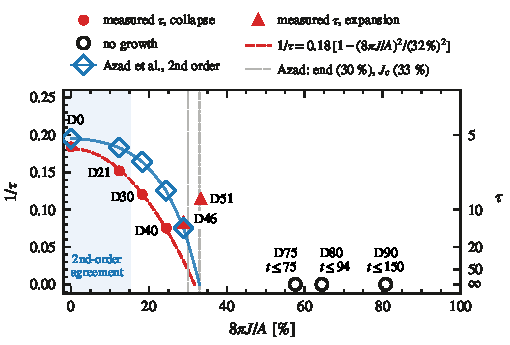
\includegraphics[width=\columnwidth]{instability_curve.pdf}
\caption{Inverse $e$-fold time $1/\tau$ of the throat's areal radius against the angular momentum as a fraction of its extremal value (Table~\ref{tab:results}), beside the second-order rates of Refs.~\cite{azad2023,azad2024} ($J_c$: the zero of their rate). The rates follow second order at slow spin and fall below it at higher spin; near $30\%$ the unperturbed throat expands instead of collapsing.}
\label{fig:curve}
\end{figure}

% Figs. 4 and 5 are read here, a page early, so that each heads a page of text.
\begin{figure*}[t]
\centering
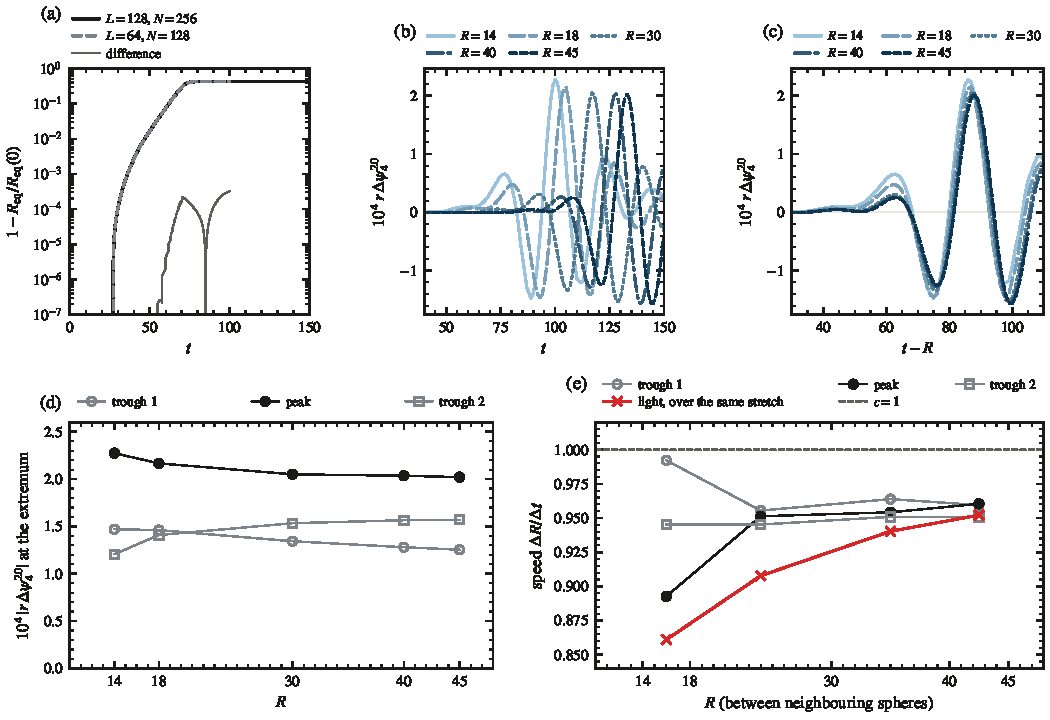
\includegraphics[width=\textwidth]{farzone_wave_02c.pdf}
\caption{The $(2,0)$ wave of the unperturbed rotating collapse. (a)~$r\,\Delta\psi_4^{20}$ of the D21 run on the $L=128$ box, on spheres $R=14$--45 against retarded time $t-R$; only the first lobe falls with $R$ (near field). (b)~The wave against spin at $R=14$, each run on its own collapse clock $u=t-R-t_{10}$ ($t_{10}$: the time its equatorial deficit passes $10\%$); the static run (D0) is drawn at zero, its measured record below $3\times10^{-8}$. (c)~The radiated energy $E_{20}=\tfrac{1}{16\pi}\int|\int r\psi_4\,dt'|^{2}\,dt$ over the aligned burst, per unit $M_{\rm ADM}$, at $R=18$ (filled) and $R=14$ (open). (d)~The speed of each extremum between neighbouring spheres, against the local coordinate speed of light (crosses). The burst's energy grows with spin, and the static collapse radiates nothing.}
\label{fig:wave}
\end{figure*}


Evolution uses \texttt{GRTeclyn}~\cite{grteclyn,amrex,grchombo} with the setup of Refs.~\cite{shirokov2026,shirokov2026c}: the CCZ4 formulation of the Einstein equations~\cite{alic2012}, $1{+}\log$ slicing~\cite{bona1995}, Gamma-driver shift~\cite{alcubierre2003gauge}, fourth-order stencils, fourth-order Runge--Kutta time integration with $\Delta t=0.02\,\Delta x$ in every run, Kreiss--Oliger dissipation of strength $\sigma$, and a floored conformal factor at the puncture. The only scheme parameter that varies between runs is $\sigma$ (Table~\ref{tab:ladder}): the larger value suppresses a grid-scale mode that grows at the fixed mesh-refinement interfaces (Appendix~\ref{app:interface}). The larger $\sigma$ smooths the initial data more and advances the collapse by about 4 time units, so we compare rates only at equal $\sigma$.

\subsection{Long evolutions: the outer boundary}
\label{sec:setup:boundary}

Evolutions that must outlive the outer-boundary crossing time $t\approx L$ need an outer boundary that neither reflects nor drives the interior. Kreiss--Oliger dissipation cannot do it, since its strength falls as the sixth power of wavelength, so the sponge layer of Refs.~\cite{shirokov2026,shirokov2026c} is transparent to the long outgoing gauge pulse; and a flat-space Sommerfeld condition assumes asymptotics the wormhole does not have (mass 1--12 sits inside the box). Two changes in the same outer layer fix it. The Sommerfeld condition is imposed on the deviation of the evolved fields from the stationary background rather than on the fields themselves; and a damping layer can in addition drive every evolved field back to that background at rate $\lambda$, $\partial_t u \to \partial_t u - \lambda\,f(r)\,(u-u_{\rm bg})$, with $f(r)$ the sponge's quartic ramp and $u_{\rm bg}$ the run's own initial data, rebuilt exactly from the background tables; $\lambda=0$ recovers the base scheme identically. The layer is validated at $\lambda=1$ on the static drainhole against the reference evolution: the trace $K$ of the extrinsic curvature falls two orders of magnitude across the layer, while everything inside it (the throat radii to four digits, the constraint norms, the near-zone $\Psi_4$ signal) is unchanged, so it absorbs at all wavelengths without touching the interior. On the $L=64$ box, whose layer ($r=24$--32) contains the outermost extraction sphere, a side-by-side test showed the background-relative boundary alone keeps the outer levels cleaner, so those runs take the damping off; the $L=128$ boxes ($r=48$--64, outside every sphere) run with it on (Table~\ref{tab:ladder}). With the boundary treated this way the $L=64$ runs, previously reliable only to the crossing time $t\approx64$, run to their final times $t=100$--$150$, with the converged span set by the constraint norms instead.

\subsection{Criteria, diagnostics and runs}
\label{sec:setup:runs}

Stability claims follow the criteria of Sec.~II of Ref.~\cite{evstafyeva2025}: a gauge-invariant measure of the growth, for which we use the throat's areal radius and the marginally outer-trapped surface (MOTS) found spectrally on every output; constraint norms that converge at the code's order while the growth proceeds; an $e$-fold time that converges to a nonzero value across resolutions; and its dependence on the perturbation, tested at D21 with imposed perturbations of both signs ($|\varepsilon|=10^{-3}$; Table~\ref{tab:ladder}). Every run carries three nested refinement levels on the throat, and the domain size follows the model's mass: $M_{\rm ADM}$ triples along the family (1.112 at $v_e=0.21$, 3.311 at $0.70$), so the distance from the throat to the $L=64$ boundary falls from $25\,M_{\rm ADM}$ at slow spin to under $10\,M_{\rm ADM}$ at $v_e=0.70$. Models up to $v_e=0.51$ therefore run on the $L=64$, $N=128$ grid of the static evolution of Ref.~\cite{shirokov2026c}, and models from $v_e=0.59$ on $L=128$, $N=256$ at the same finest $\Delta x$. The Newman--Penrose scalar $\Psi_4$, whose multipoles carry the outgoing gravitational wave, is extracted on spheres at $R=10$--30 ($L=64$) and $R=14$--45 ($L=128$); the signal is its $(\ell,m)=(2,0)$ mode. Resolution triplets anchor the two ends of the spin sequence (Appendix~\ref{app:conv}). Table~\ref{tab:ladder} lists every run, from the static reference through the $O(J^2)$ regime~\cite{azad2023,azad2024} to far beyond any perturbative result.

\section{The instability across the spin range}
\label{sec:slow}

\begin{table*}[t]
\caption{Results of the simulations of Table~\ref{tab:ladder}, row by row. $t_{\rm conv}$: the time up to which the run is converged; nothing later is quoted, in the text or the figures. $t_{1\%}$: when the throat's areal radius first departs from its initial value by $1\%$. $\tau$: the $e$-fold time of the unstable mode (Sec.~\ref{sec:slow}). GW: the $(2,0)$ burst at $R=14$ arrives before $t_{\rm conv}$ (burst), is still rising at $t_{\rm conv}$ (onset), or stays below the extraction floor (none). MOTS: the marginally outer-trapped surface.}
\label{tab:results}
\scriptsize
\setlength{\tabcolsep}{3pt}
\begin{ruledtabular}
\begin{tabular}{llllllp{0.42\textwidth}}
model & $N$ & $t_{\rm conv}$ & $t_{1\%}$ & $\tau$ & GW & end state \\
\hline
D0 & 128 & 60 & 43.8 & 5.4 & none & collapses; ends inside the horizon \\
D21 & 96/128/192 & 55/100/100 & 41.9/46.8/57.6 & 7.8/6.6/6.1 & burst & collapses; horizon settles at $R=2.52$ \\
D21$\pm\varepsilon$ & 128 & 42/61 & 24.2/24.2 & -- & onset & outward collapses, inward expands \\
D21 & 256 & 150 & 46.8 & -- & burst & collapses; the $(2,0)$ burst on spheres $R=14$--45 (Fig.~\ref{fig:wave}) \\
D30 & 128 & 100 & 51.0 & 8.3 & burst & collapses; horizon at $R=2.571$ at $t=100$ \\
D30 & 128 & 130 & 51.0 & 8.3 & burst & collapses; horizon settles at $R=2.567$ \\
D40 & 128 & 100 & 58.7 & 13.3 & onset & collapses; MOTS leaves the throat, $t=92$ \\
D46 & 128 & 100 & 73.7 & -- & onset & $-1.12\%$ at $t=83$, turning back by $t=100$ \\
D46 & 128 & 121 & 73.7 & 12.1 & onset & expands from $t=101$ \\
D51 & 192 & 100 & 94.2 & -- & none & shrinks: the opposite perturbation sign \\
D51 & 128 & 95 & 85.8 & 8.8 & none & expands from $t\approx70$ \\
D75 & 256 & 75 & -- & -- & none & no growth: areal drift $\le6\times10^{-5}$ \\
D80 & 256 & 94 & -- & -- & none & no growth: areal drift $\le7\times10^{-5}$ \\
D90 & 128/192/256 & 150 & -- & -- & none & no growth: areal drift $\le7\times10^{-5}$ at all three $N$ \\
\end{tabular}
\end{ruledtabular}
\end{table*}


\emph{Perturbative initial data.} We first evolved the second-order $O(J^2)$ backgrounds of Ref.~\cite{azad2024} at $J=0.25$ and $J=1$ on the drainhole family. Both throats expanded where the static throat collapses: the same unstable mode with the opposite sign ($\tau=5.8$ and $5.6$). Expressed as the equivalent radial perturbation amplitude of Ref.~\cite{shirokov2026c}, however, the effective perturbation was $\varepsilon\approx-3\times10^{-5}$ at $J=0.25$ and $-7\times10^{-3}$ at $J=1$: growth by a factor ${\sim}230$ for a factor 4 in $J$, i.e.\ ${\sim}J^4$, the size of the $O(J^2)$ data's own truncation error, which the independent Einstein residual puts at $10^{-2}$ at $J=1$ (Sec.~\ref{sec:solver}). Second-order data trigger the very instability under study at their own error level; nothing at slow spin can be concluded from them.

\emph{Measuring the growth.} The diagnostic for every unperturbed evolution is the throat's areal radius $R_A(t)$, the size of the $\ell=0$ mode the perturbative work computes. The $e$-fold time is an offset-free fit: the slope of $\ln|dR_A/dt|$ over the span where the areal deficit $1-R_A(t)/R_A(0)$ (collapse) or growth (expansion) first passes 0.2--1\%. Fitting the rate of change rather than the deficit itself removes the initial transient's baseline, which biases a direct log fit of the deficit by a resolution-dependent amount. The band sits on a plateau: the measured $\tau$ moves by under $4\%$ between the 0.2--1\% and 0.5--2\% bands. So measured, $\tau$ self-converges across the D21 resolution triplet, 7.8, 6.6 and 6.1 at $N=96$, 128 and 192, at third to fourth order ($Q=2.3$; Appendix~\ref{app:conv}); Richardson extrapolation at that measured order gives the continuum value $\tau=5.9$. The finite-resolution bias is close to a common factor on every rate, so it cancels in the zero of the fit below.

\emph{The collapse branch.} On the spectral backgrounds the behaviour reverses: the unperturbed throat collapses on the static mode, later and more slowly the faster it spins. Along the models D0--D40 the time at which the areal radius has fallen by $1\%$ grows steadily, and $\tau$ rises from 5.4 to 13.3 (Fig.~\ref{fig:curve}; Table~\ref{tab:results}). Each collapse ends in a black hole: the D21 horizon settles at $R=2.524$ (irreducible mass $M_{\rm irr}=R/2=1.26$), the D30 at $R=2.567$ by $t=130$; the D40's MOTS leaves the throat at $t=92$ and reads $R=3.22$, still shrinking, at $t=100$. Each evolution is perturbed only by its own discretization error; because $\tau$ comes from the growth rate, it does not depend on the perturbation amplitude, which differs between runs.

\emph{The expanding branch.} At $v_e=0.456$ ($28.8\%$ of extremal) the unperturbed throat expands instead: the areal radius falls by $1.12\%$ by $t=83$, turns, crosses zero at $t=101$ and grows exponentially, $\tau=12.1$. The D51 model behaves the same way ($-0.30\%$ at $t=65$--68, then exponential growth with $\tau=8.8$), and the MOTS is lost once a throat expands: no trapped surface forms. Collapse and expansion are the instability's two end states, and the sign of the initial perturbation selects between them. The imposed radial perturbations at D21 show it directly: under an inward perturbation the throat expands, under an outward one it collapses, and both depart by $1\%$ at $t\approx24$ at the same rate. The D51 run whose absorbing layer gives the opposite effective perturbation shrinks instead. The end state of D51 thus depends on the outer-boundary treatment, and classifying the branch at this spin needs explicit control of the perturbation sign. At the fast end, the D75 and D80 throat radii show no growth within their converged spans (areal drift $\le7\times10^{-5}$), and the D90 throat radius shows no growth up to $t=150$, about 28 $e$-folding times of the static mode, at all three resolutions (Appendix~\ref{app:conv}). Between D51 and D75 the compactified far end breaks down before the throat's behaviour can be measured (the shaded band of Fig.~\ref{fig:trends}c).

\emph{Against the perturbative prediction.} Figure~\ref{fig:curve} puts both branches on one axis. Where second order should hold, the two methods are close: the D21 continuum rate lies within $8\%$ of the second-order $C=1$ value of Refs.~\cite{azad2023,azad2024} ($\tau=5.9$ against 5.46), and the static member lies beside its linear mode (5.4 at $N=128$, extrapolating toward 5.1). At intermediate spin the measured mode is slower than their second-order values by more than the resolution bias ($\tau=8.3$ against 6.1 at $v_e=0.30$, 13.3 against 8.0 at 0.40), a gap that grows with spin, as expected if the neglected $O(J^4)$ terms become important. The collapse branch itself follows $a-b\,(J/A)^2$ to rms $2\times10^{-3}$ in $1/\tau$ and extrapolates to zero at $32\%$ of the extremal angular momentum, beside the zero of their second-order rate ($33\%$) and their conjectured mode crossing (${\approx}30\%$). The instability nevertheless does not end there: the $28.8\%$ and $33\%$ models expand with rates that rise with spin ($\tau=12.1$, then 8.8), consistent with their second unstable mode taking over rather than the two modes merging away. Their $\tau$ is a linear mode in Killing time, ours a nonlinear areal-radius fit, so the pointwise comparison is indicative.

\emph{Gravitational waves.} The rotating collapse radiates with no nonspherical perturbation put in (Fig.~\ref{fig:wave}): a single $(2,0)$ burst with ring-down period ${\approx}24$, propagating at the local light speed, its extrema flat in extraction radius to $1.5\%$ over $R=30$--45 on the $L=128$ box, which reproduces the $L=64$ throat history to $3\times10^{-4}$. Aligned on each model's own collapse, the D30 burst has the D21's shape and timing at about 1.5 times the amplitude, and the radiated energy per unit mass grows as the amplitude squared, $E_{20}/M_{\rm ADM}=3.3\times10^{-7}\to8.0\times10^{-7}$. The spherical static collapse radiates nothing: its measured record stays below $3\times10^{-8}$. Rotation thus imprints itself on the burst a collapsing throat emits, before any horizon forms.

\section{Conclusions}
\label{sec:conclusions}

First, the spinning Ellis--Bronnikov parameter space is now available as tabulated solutions: both families from slow rotation to $v_e\approx0.99$, including the drainhole family for which nothing was published, with the published $\nu$ equation, Eq.~(12) of Ref.~\cite{chew2016}, corrected to Eq.~\eqref{eq:nueq}. The practical lesson generalizes: a solver checked only against the equations it imposes would have passed every test while solving a different system; the unimposed identities caught the difference. Second, the pipeline from these solutions to 3+1 evolution is validated at fourth order, and $O(J^2)$ initial data are shown to be unsuitable for stability work: their truncation error triggers the instability itself. Third, the nonlinear evolutions show the instability slowing and then changing branch. The radial collapse slows with spin ($\tau=5.4\to13.3$ from the static model to $24\%$ of the extremal angular momentum), its rate following $a-b\,(J/A)^2$, which extrapolates to zero at $32\%$, beside the second-order prediction of $33\%$~\cite{azad2023,azad2024}. Near $30\%$, where the perturbative mode crossing was conjectured to end the instability, the unperturbed throat expands instead, with a rate that rises with spin. From $58\%$ of the extremal angular momentum upward the throat shows no growth within the converged spans; at $81\%$ this holds to $t=150$, about 28 $e$-folding times of the static mode, at three resolutions, addressing, for this family and timescale, the four-dimensional stability question left open in Ref.~\cite{kleihaus_kunz2014}. The rotating collapse also radiates a $(2,0)$ burst from unperturbed, axisymmetric data, its energy growing with spin as the amplitude squared, while the static collapse radiates nothing.

These conclusions carry their limits. The evolutions end at $t\le150$, so they bound growth only over that span; a slower mode could still emerge later. Above about $29\%$ of the extremal angular momentum ($v_e\approx0.46$) the throat's equator lies inside an ergoregion. Horizonless rotating objects with an ergoregion are generically subject to a slow nonaxisymmetric instability~\cite{friedman1978,cardoso2008}; our runs, started from axisymmetric data, bound only axisymmetric growth. Between $33\%$ and $58\%$ the far end fails before the throat's behaviour can be measured, so that band is unmeasured. Only the drainhole family ($C=1$) was evolved; the symmetric family enters through the solver validation alone. The end state of each unperturbed run is set by the sign of its effective perturbation, so collapse and expansion label the sign of that perturbation, not the model. And the $32\%$ zero is an extrapolation of the collapse-branch fit beyond the last collapsing model at $24\%$, not a measured endpoint.

\section{Reproducibility and cost}
\label{sec:data}

The solver, the evolution code and the figure scripts are available at \url{https://github.com/Nikchik-coder/GRTeclyn} (branch \texttt{feature/spinning}). Its directory \texttt{results/spinningwormhole} holds the solver's accepted solutions, the headers of the background tables the evolutions start from, and every evolution's parameter file and diagnostic time series.

Every evolution ran on one NVIDIA H100 80\,GB device, with \texttt{GRTeclyn} built CUDA-native against AMReX~26.02. A run on the $L=64$, $N=128$ grid takes 7.6--11.1\,h to $t=100$; the $N=192$ members 20\,h, peaking at 53\,GiB; the $L=128$, $N=256$ runs 9.7\,h to $t=150$. The 19 evolutions of Table~\ref{tab:ladder} took 185 GPU-hours.

\begin{acknowledgments}
This work was supported by Gravity Frontiers
(\url{https://www.gravityfrontiers.org/en}), which funded the underlying
research and the development of the numerical-simulation software. The authors
acknowledge the GRTL Collaboration for \texttt{GRChombo}, \texttt{GRTresna},
and \texttt{GRTeclyn}.
\end{acknowledgments}

\appendix

\section{Convergence of the evolutions}
\label{app:conv}

The two resolution triplets are D21, the slowest spinning collapse (Fig.~\ref{fig:conv02}), and D90, the stable fast model (Fig.~\ref{fig:conv09}), both read through the per-level constraint norms of Appendix~\ref{app:interface}. Rescaling constraint norms between resolutions is a valid convergence test because their exact value is zero. For the D21 triplet's grid spacings ($h\propto1/N$, $N=96/128/192$) the expected self-convergence factors $Q_n=(h_1^{\,n}-h_2^{\,n})/(h_2^{\,n}-h_3^{\,n})$ are $Q_3=1.95$ and $Q_4=2.69$; the offset-free growth rate of Sec.~\ref{sec:slow} measures $Q=2.3$, converging at the same order as the constraints.

% Both figures share one float page after the appendix text (\packfloatpages
% stacks them from its top); the \FloatBarrier before the references puts
% that page ahead of them.
\packfloatpages

\begin{figure*}[tp]
\centering
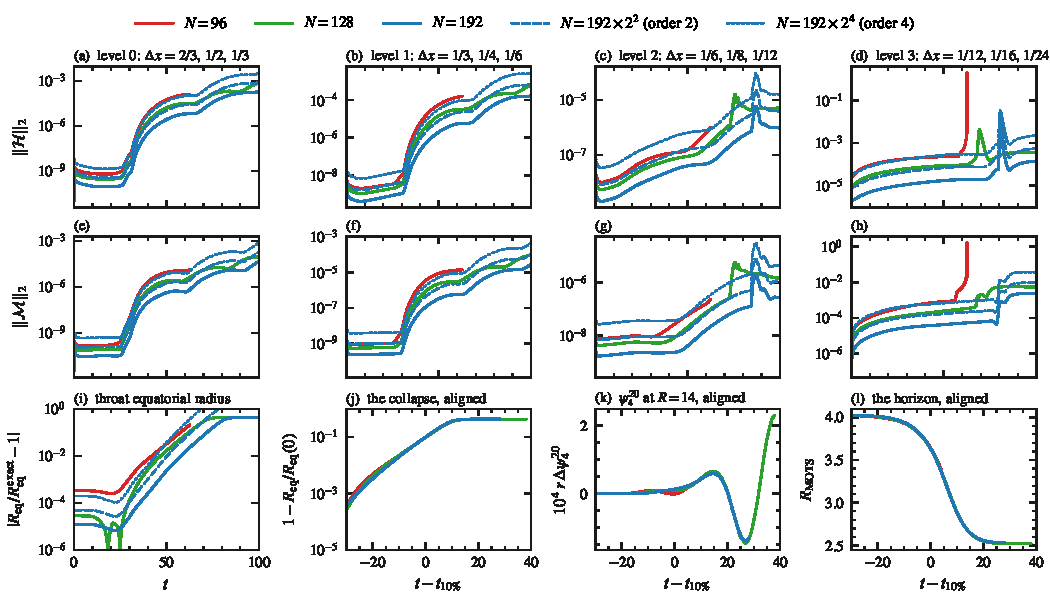
\includegraphics[width=0.82\textwidth]{convergence_02c.pdf}
\caption{Convergence of the D21 model over its triplet $N=96/128/192$ ($L=64$; finest $\Delta x$ in each panel title). (a)--(d)~Hamiltonian and (e)--(h)~momentum constraint norms per refinement level; dashed and dotted, the $N=192$ norms rescaled by $2^{2}$ and $2^{4}$: the measured $N=96$ norms lie between the second- and fourth-order brackets on every level while the collapse grows. (i)~The equatorial throat radius against the stationary solution, falling with resolution. (j)~The collapse, each run aligned at its own $10\%$ time: the three resolutions land on one curve. (k)~$r\,\Delta\psi_4^{20}$ at $R=14$, aligned: $N=128$ and 192 overlap ($N=96$ dies in its collapse before the burst arrives). (l)~The MOTS radius, aligned: one horizon, settling at $R=2.52$. The collapse rate self-converges at third to fourth order ($Q=2.3$); the waveform and the horizon agree across resolutions.}
\label{fig:conv02}
\end{figure*}

\begin{figure*}[tp]
\centering
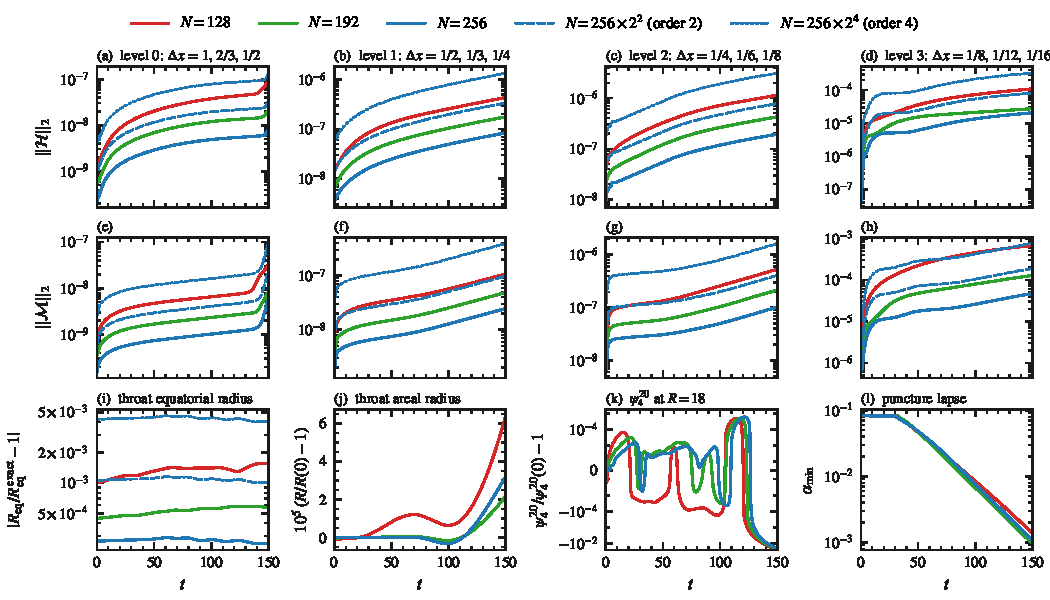
\includegraphics[width=0.82\textwidth]{convergence_09c.pdf}
\caption{Stability of the D90 model over its triplet $N=128/192/256$ ($L=128$; finest $\Delta x$ in each panel title), to $t=150$. (a)--(h)~Constraint norms per level with the same second-/fourth-order brackets as Fig.~\ref{fig:conv02}: every level converges with resolution over the run. (i)~The equatorial throat radius holds the stationary value, its offset falling with resolution. (j)~The areal throat radius drifts by $\le7\times10^{-5}$ over the full run. (k)~The $(2,0)$ extraction at $R=18$, relative to its $t=0$ read-off: fluctuations at the $10^{-4}$ level, no burst. (l)~The lapse at the $\eta\to-\infty$ puncture falls smoothly at all three resolutions (the gauge, not the geometry). The D90 throat shows no growing radius and no wave at any resolution over the run, with constraint norms converging.}
\label{fig:conv09}
\end{figure*}

\section{The refinement-interface mode and the timestep}
\label{app:interface}

The timestep $\Delta t=0.02\,\Delta x$ was adopted empirically in Refs.~\cite{shirokov2026,shirokov2026c}. We traced what sets it to a grid-scale mode pinned to the fixed coarse--fine interfaces of the nested refinement boxes, dissipation-starved at $\sigma=0.1$, whose growth rate rises with the timestep. Constraint norms evaluated per refinement level, with cells covered by finer levels masked, expose the mode by $t\approx10$; the domain-wide norm is blind to it until breakout. Raising the dissipation where the mode lives removes it: at $\sigma=0.4$ the interface-level norms sit $10^{2}$--$10^{4}$ below the $\sigma=0.1$ reference by $t=100$. The larger timesteps this would permit do not transfer to the spinning backgrounds, which lose the $\eta\to-\infty$ region (the puncture) by $t\approx22$--48 at $\Delta t=0.035$--$0.05\,\Delta x$, so the production runs take no speed-up.

% No float may land inside the reference list: a figure still held here is
% placed before it.
\FloatBarrier

\begin{thebibliography}{99}

\bibitem{ellis1973}
H.~G.~Ellis,
\newblock ``Ether flow through a drainhole: A particle model in general relativity,''
\newblock J.\ Math.\ Phys.\ \textbf{14}, 104 (1973).

\bibitem{bronnikov1973}
K.~A.~Bronnikov,
\newblock ``Scalar-tensor theory and scalar charge,''
\newblock Acta Phys.\ Polon.\ B \textbf{4}, 251 (1973).

\bibitem{morris_thorne1988}
M.~S.~Morris and K.~S.~Thorne,
\newblock ``Wormholes in spacetime and their use for interstellar travel: A tool for teaching general relativity,''
\newblock Am.\ J.\ Phys.\ \textbf{56}, 395 (1988).

\bibitem{visser1995}
M.~Visser,
\newblock \emph{Lorentzian Wormholes: From Einstein to Hawking}
\newblock (AIP Press, Woodbury, NY, 1995).

\bibitem{gonzalez2009lin}
J.~A.~Gonz\'alez, F.~S.~Guzm\'an, and O.~Sarbach,
\newblock ``Instability of wormholes supported by a ghost scalar field. I. Linear stability analysis,''
\newblock Class.\ Quantum Grav.\ \textbf{26}, 015010 (2009).

\bibitem{gonzalez2009}
J.~A.~Gonz\'alez, F.~S.~Guzm\'an, and O.~Sarbach,
\newblock ``Instability of wormholes supported by a ghost scalar field. II. Nonlinear evolution,''
\newblock Class.\ Quantum Grav.\ \textbf{26}, 015011 (2009).

\bibitem{shinkai2002}
H.~Shinkai and S.~A.~Hayward,
\newblock ``Fate of the first traversible wormhole: Black-hole collapse or inflationary expansion,''
\newblock Phys.\ Rev.\ D \textbf{66}, 044005 (2002).

\bibitem{bronnikov2011}
K.~A.~Bronnikov, J.~C.~Fabris, and A.~Zhidenko,
\newblock ``On the stability of scalar-vacuum space-times,''
\newblock Eur.\ Phys.\ J.\ C \textbf{71}, 1791 (2011).

\bibitem{cremona2019}
F.~Cremona, F.~Pirotta, and L.~Pizzocchero,
\newblock ``On the linear instability of the Ellis--Bronnikov--Morris--Thorne wormhole,''
\newblock Gen.\ Relativ.\ Gravit.\ \textbf{51}, 19 (2019).

\bibitem{shirokov2026}
N.~M.~Shirokov,
\newblock ``Wormhole dynamics: nonlinear collapse and gravitational-wave emission,''
\newblock arXiv:2604.00071 [gr-qc] (2026).

\bibitem{shirokov2026c}
N.~M.~Shirokov and I.~Nachevsky,
\newblock ``Binary Ellis--Bronnikov wormholes in 3+1 numerical relativity: mergers, fly-bys and gravitational waves,''
\newblock arXiv:2610.13206 [gr-qc] (2026).

\bibitem{matos2006}
T.~Matos and D.~N\'u\~nez,
\newblock ``Rotating scalar field wormhole,''
\newblock Class.\ Quantum Grav.\ \textbf{23}, 4485 (2006).

\bibitem{kashargin2008}
P.~E.~Kashargin and S.~V.~Sushkov,
\newblock ``Slowly rotating wormholes: The first order approximation,''
\newblock Grav.\ Cosmol.\ \textbf{14}, 80 (2008);
\newblock ``Slowly rotating scalar field wormholes: The second order approximation,''
\newblock Phys.\ Rev.\ D \textbf{78}, 064071 (2008).

\bibitem{kleihaus_kunz2014}
B.~Kleihaus and J.~Kunz,
\newblock ``Rotating Ellis wormholes in four dimensions,''
\newblock Phys.\ Rev.\ D \textbf{90}, 121503(R) (2014).

\bibitem{chew2016}
X.~Y.~Chew, B.~Kleihaus, and J.~Kunz,
\newblock ``Geometry of spinning Ellis wormholes,''
\newblock Phys.\ Rev.\ D \textbf{94}, 104031 (2016).

\bibitem{volkov2021}
M.~S.~Volkov,
\newblock ``Stationary generalizations for the Bronnikov--Ellis wormhole and for the vacuum ring wormhole,''
\newblock Phys.\ Rev.\ D \textbf{104}, 124064 (2021).

\bibitem{azad2023}
B.~Azad, J.~L.~Bl\'azquez-Salcedo, F.~S.~Khoo, and J.~Kunz,
\newblock ``Are slowly rotating Ellis--Bronnikov wormholes stable?,''
\newblock Phys.\ Lett.\ B \textbf{848}, 138349 (2024).

\bibitem{azad2024}
B.~Azad, J.~L.~Bl\'azquez-Salcedo, F.~S.~Khoo, and J.~Kunz,
\newblock ``Radial perturbations of Ellis--Bronnikov wormholes in slow rotation up to second order,''
\newblock Phys.\ Rev.\ D \textbf{109}, 124051 (2024).

\bibitem{dzhunushaliev2013}
V.~Dzhunushaliev, V.~Folomeev, B.~Kleihaus, J.~Kunz, and E.~Radu,
\newblock ``Rotating wormholes in five dimensions,''
\newblock Phys.\ Rev.\ D \textbf{88}, 124028 (2013).

\bibitem{blazquez2025}
J.~L.~Bl\'azquez-Salcedo, L.~M.~Gonz\'alez-Romero, F.~S.~Khoo, J.~Kunz, and P.~Navarro Moreno,
\newblock ``Radial perturbations of charged wormholes,''
\newblock arXiv:2510.11406 [gr-qc] (2025).

\bibitem{visser2003}
M.~Visser, S.~Kar, and N.~Dadhich,
\newblock ``Traversable wormholes with arbitrarily small energy condition violations,''
\newblock Phys.\ Rev.\ Lett.\ \textbf{90}, 201102 (2003).

\bibitem{khoo2024}
F.~S.~Khoo \emph{et al.},
\newblock ``Quasinormal modes of rapidly rotating Ellis--Bronnikov wormholes,''
\newblock Phys.\ Rev.\ D \textbf{109}, 084013 (2024).

\bibitem{evstafyeva2025}
T.~Evstafyeva, N.~Siemonsen, and W.~E.~East,
\newblock ``Assessing the stability of ultracompact spinning boson stars with nonlinear evolutions,''
\newblock arXiv:2508.11527 [gr-qc] (2025).

\bibitem{alic2012}
D.~Alic, C.~Bona-Casas, C.~Bona, L.~Rezzolla, and C.~Palenzuela,
\newblock ``Conformal and covariant formulation of the Z4 system with constraint-violation damping,''
\newblock Phys.\ Rev.\ D \textbf{85}, 064040 (2012).

\bibitem{bona1995}
C.~Bona, J.~Mass\'o, E.~Seidel, and J.~Stela,
\newblock ``New formalism for numerical relativity,''
\newblock Phys.\ Rev.\ Lett.\ \textbf{75}, 600 (1995).

\bibitem{alcubierre2003gauge}
M.~Alcubierre, B.~Br\"ugmann, P.~Diener, M.~Koppitz, D.~Pollney, E.~Seidel, and R.~Takahashi,
\newblock ``Gauge conditions for long-term numerical black hole evolutions without excision,''
\newblock Phys.\ Rev.\ D \textbf{67}, 084023 (2003).

\bibitem{grteclyn}
GRTL Collaboration,
\newblock \texttt{GRTeclyn},
\newblock \url{https://github.com/GRTLCollaboration/GRTeclyn}.

\bibitem{amrex}
W.~Zhang \emph{et al.},
\newblock ``AMReX: a framework for block-structured adaptive mesh refinement,''
\newblock J.\ Open Source Softw.\ \textbf{4}, 1370 (2019).

\bibitem{grchombo}
T.~Andrade \emph{et al.},
\newblock ``GRChombo: an adaptable numerical relativity code for fundamental physics,''
\newblock J.\ Open Source Softw.\ \textbf{6}, 3703 (2021).

\bibitem{friedman1978}
J.~L.~Friedman,
\newblock ``Ergosphere instability,''
\newblock Commun.\ Math.\ Phys.\ \textbf{63}, 243 (1978).

\bibitem{cardoso2008}
V.~Cardoso, P.~Pani, M.~Cadoni, and M.~Cavagli\`a,
\newblock ``Ergoregion instability of ultracompact astrophysical objects,''
\newblock Phys.\ Rev.\ D \textbf{77}, 124044 (2008).

\end{thebibliography}

\end{document}
